% Options for packages loaded elsewhere
\PassOptionsToPackage{unicode}{hyperref}
\PassOptionsToPackage{hyphens}{url}
%
\documentclass[
]{article}
\usepackage{amsmath,amssymb}
\usepackage{iftex}
\ifPDFTeX
  \usepackage[T1]{fontenc}
  \usepackage[utf8]{inputenc}
  \usepackage{textcomp} % provide euro and other symbols
\else % if luatex or xetex
  \usepackage{unicode-math} % this also loads fontspec
  \defaultfontfeatures{Scale=MatchLowercase}
  \defaultfontfeatures[\rmfamily]{Ligatures=TeX,Scale=1}
\fi
\usepackage{lmodern}
\ifPDFTeX\else
  % xetex/luatex font selection
\fi
% Use upquote if available, for straight quotes in verbatim environments
\IfFileExists{upquote.sty}{\usepackage{upquote}}{}
\IfFileExists{microtype.sty}{% use microtype if available
  \usepackage[]{microtype}
  \UseMicrotypeSet[protrusion]{basicmath} % disable protrusion for tt fonts
}{}
\makeatletter
\@ifundefined{KOMAClassName}{% if non-KOMA class
  \IfFileExists{parskip.sty}{%
    \usepackage{parskip}
  }{% else
    \setlength{\parindent}{0pt}
    \setlength{\parskip}{6pt plus 2pt minus 1pt}}
}{% if KOMA class
  \KOMAoptions{parskip=half}}
\makeatother
\usepackage{xcolor}
\usepackage[margin=1in]{geometry}
\usepackage{color}
\usepackage{fancyvrb}
\newcommand{\VerbBar}{|}
\newcommand{\VERB}{\Verb[commandchars=\\\{\}]}
\DefineVerbatimEnvironment{Highlighting}{Verbatim}{commandchars=\\\{\}}
% Add ',fontsize=\small' for more characters per line
\usepackage{framed}
\definecolor{shadecolor}{RGB}{248,248,248}
\newenvironment{Shaded}{\begin{snugshade}}{\end{snugshade}}
\newcommand{\AlertTok}[1]{\textcolor[rgb]{0.94,0.16,0.16}{#1}}
\newcommand{\AnnotationTok}[1]{\textcolor[rgb]{0.56,0.35,0.01}{\textbf{\textit{#1}}}}
\newcommand{\AttributeTok}[1]{\textcolor[rgb]{0.13,0.29,0.53}{#1}}
\newcommand{\BaseNTok}[1]{\textcolor[rgb]{0.00,0.00,0.81}{#1}}
\newcommand{\BuiltInTok}[1]{#1}
\newcommand{\CharTok}[1]{\textcolor[rgb]{0.31,0.60,0.02}{#1}}
\newcommand{\CommentTok}[1]{\textcolor[rgb]{0.56,0.35,0.01}{\textit{#1}}}
\newcommand{\CommentVarTok}[1]{\textcolor[rgb]{0.56,0.35,0.01}{\textbf{\textit{#1}}}}
\newcommand{\ConstantTok}[1]{\textcolor[rgb]{0.56,0.35,0.01}{#1}}
\newcommand{\ControlFlowTok}[1]{\textcolor[rgb]{0.13,0.29,0.53}{\textbf{#1}}}
\newcommand{\DataTypeTok}[1]{\textcolor[rgb]{0.13,0.29,0.53}{#1}}
\newcommand{\DecValTok}[1]{\textcolor[rgb]{0.00,0.00,0.81}{#1}}
\newcommand{\DocumentationTok}[1]{\textcolor[rgb]{0.56,0.35,0.01}{\textbf{\textit{#1}}}}
\newcommand{\ErrorTok}[1]{\textcolor[rgb]{0.64,0.00,0.00}{\textbf{#1}}}
\newcommand{\ExtensionTok}[1]{#1}
\newcommand{\FloatTok}[1]{\textcolor[rgb]{0.00,0.00,0.81}{#1}}
\newcommand{\FunctionTok}[1]{\textcolor[rgb]{0.13,0.29,0.53}{\textbf{#1}}}
\newcommand{\ImportTok}[1]{#1}
\newcommand{\InformationTok}[1]{\textcolor[rgb]{0.56,0.35,0.01}{\textbf{\textit{#1}}}}
\newcommand{\KeywordTok}[1]{\textcolor[rgb]{0.13,0.29,0.53}{\textbf{#1}}}
\newcommand{\NormalTok}[1]{#1}
\newcommand{\OperatorTok}[1]{\textcolor[rgb]{0.81,0.36,0.00}{\textbf{#1}}}
\newcommand{\OtherTok}[1]{\textcolor[rgb]{0.56,0.35,0.01}{#1}}
\newcommand{\PreprocessorTok}[1]{\textcolor[rgb]{0.56,0.35,0.01}{\textit{#1}}}
\newcommand{\RegionMarkerTok}[1]{#1}
\newcommand{\SpecialCharTok}[1]{\textcolor[rgb]{0.81,0.36,0.00}{\textbf{#1}}}
\newcommand{\SpecialStringTok}[1]{\textcolor[rgb]{0.31,0.60,0.02}{#1}}
\newcommand{\StringTok}[1]{\textcolor[rgb]{0.31,0.60,0.02}{#1}}
\newcommand{\VariableTok}[1]{\textcolor[rgb]{0.00,0.00,0.00}{#1}}
\newcommand{\VerbatimStringTok}[1]{\textcolor[rgb]{0.31,0.60,0.02}{#1}}
\newcommand{\WarningTok}[1]{\textcolor[rgb]{0.56,0.35,0.01}{\textbf{\textit{#1}}}}
\usepackage{graphicx}
\makeatletter
\def\maxwidth{\ifdim\Gin@nat@width>\linewidth\linewidth\else\Gin@nat@width\fi}
\def\maxheight{\ifdim\Gin@nat@height>\textheight\textheight\else\Gin@nat@height\fi}
\makeatother
% Scale images if necessary, so that they will not overflow the page
% margins by default, and it is still possible to overwrite the defaults
% using explicit options in \includegraphics[width, height, ...]{}
\setkeys{Gin}{width=\maxwidth,height=\maxheight,keepaspectratio}
% Set default figure placement to htbp
\makeatletter
\def\fps@figure{htbp}
\makeatother
\setlength{\emergencystretch}{3em} % prevent overfull lines
\providecommand{\tightlist}{%
  \setlength{\itemsep}{0pt}\setlength{\parskip}{0pt}}
\setcounter{secnumdepth}{-\maxdimen} % remove section numbering
\ifLuaTeX
  \usepackage{selnolig}  % disable illegal ligatures
\fi
\usepackage{bookmark}
\IfFileExists{xurl.sty}{\usepackage{xurl}}{} % add URL line breaks if available
\urlstyle{same}
\hypersetup{
  pdftitle={Problem Set 2},
  pdfauthor={Group 2},
  hidelinks,
  pdfcreator={LaTeX via pandoc}}

\title{Problem Set 2}
\author{Group 2}
\date{March 21, 2026}

\begin{document}
\maketitle

\paragraph{Academic Integrity Pledge}\label{academic-integrity-pledge}

This activity is intended to assess our own understanding of the lesson.
We affirm that we will complete this problem set \textbf{independently}
and will not use \textbf{Artificial Intelligence tools (such as ChatGPT,
Copilot, Gemini, or similar systems)} to generate answers or solutions.

We will rely only on \emph{notes, textbook, and class materials} unless
otherwise permitted by the instructor. We understand that submitting
work generated or assisted by AI \textbf{violates academic integrity}
and may result in disciplinary action under university policies.

\begin{center}\rule{0.5\linewidth}{0.5pt}\end{center}

\paragraph{1.}\label{section}

\textbf{Name:} Abangan, Elijah Kahlil Andres P.

\textbf{Signature:}

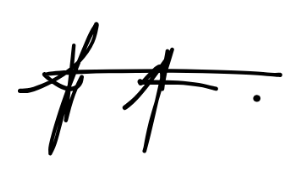
\includegraphics[width=0.1\linewidth]{Abangan_sign}

\paragraph{2.}\label{section-1}

\textbf{Name:} Barago, Sharly Pia Rose S.

\textbf{Signature:}


\includegraphics[width=0.1\linewidth]{Barago_sign}

\paragraph{3.}\label{section-2}

\textbf{Name:} Go, Andrei Benedict A.

\textbf{Signature:}


\includegraphics[width=0.05\linewidth]{Go_sign}

\paragraph{4.}\label{section-3}

\textbf{Name:} Muñoz, Nash Adam G.

\textbf{Signature:}


\includegraphics[width=0.05\linewidth]{Munoz_sign}

\paragraph{5.}\label{section-4}

\textbf{Name:} Pastoriza, Alniño Manwil E.

\textbf{Signature:}

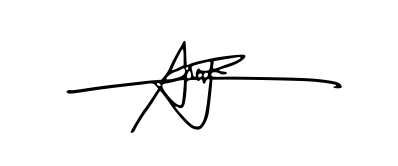
\includegraphics[width=0.1\linewidth]{Pastoriza_sign}

\paragraph{\texorpdfstring{1.) Use the bisection method with a hand
calculator or computer to find the real root of \(x^3 - x - 3 = 0\). Use
an error tolerance of \(\epsilon = 0.0001\). Graph the function
\(f(x) = x^3 - x - 3\) and label the
root.}{1.) Use the bisection method with a hand calculator or computer to find the real root of x\^{}3 - x - 3 = 0. Use an error tolerance of \textbackslash epsilon = 0.0001. Graph the function f(x) = x\^{}3 - x - 3 and label the root.}}\label{use-the-bisection-method-with-a-hand-calculator-or-computer-to-find-the-real-root-of-x3---x---3-0.-use-an-error-tolerance-of-epsilon-0.0001.-graph-the-function-fx-x3---x---3-and-label-the-root.}

\textbf{Solution:}

Finding the root using bisection, given \([a,b]=[1,2]\).

\begin{Shaded}
\begin{Highlighting}[]
\NormalTok{f\_x }\OtherTok{\textless{}{-}} \ControlFlowTok{function}\NormalTok{(x)\{x}\SpecialCharTok{\^{}}\DecValTok{3}\SpecialCharTok{{-}}\NormalTok{x}\DecValTok{{-}3}\NormalTok{\}}
\NormalTok{a }\OtherTok{\textless{}{-}} \DecValTok{1}
\NormalTok{b }\OtherTok{\textless{}{-}} \DecValTok{2}
\NormalTok{tol }\OtherTok{\textless{}{-}} \FloatTok{0.0001}

\NormalTok{bisection\_table }\OtherTok{\textless{}{-}} \FunctionTok{list}\NormalTok{(}
  \StringTok{"Iteration"} \OtherTok{=} \FunctionTok{c}\NormalTok{(),}
  \StringTok{"a"} \OtherTok{=} \FunctionTok{c}\NormalTok{(),}
  \StringTok{"b"} \OtherTok{=} \FunctionTok{c}\NormalTok{(),}
  \StringTok{"c"} \OtherTok{=} \FunctionTok{c}\NormalTok{(),}
  \StringTok{"f\_c"} \OtherTok{=} \FunctionTok{c}\NormalTok{(),}
  \StringTok{"Err."} \OtherTok{=} \FunctionTok{c}\NormalTok{()}
\NormalTok{)}

\CommentTok{\# Bisection Method Algorithm}
\NormalTok{iters }\OtherTok{\textless{}{-}} \DecValTok{1}
\ControlFlowTok{repeat}\NormalTok{ \{}
\NormalTok{  c }\OtherTok{\textless{}{-}}\NormalTok{ (a }\SpecialCharTok{+}\NormalTok{ b) }\SpecialCharTok{/} \DecValTok{2}
\NormalTok{  abs\_err }\OtherTok{\textless{}{-}} \FunctionTok{abs}\NormalTok{(b }\SpecialCharTok{{-}}\NormalTok{ c)}
\NormalTok{  f\_c }\OtherTok{\textless{}{-}} \FunctionTok{f\_x}\NormalTok{(c)}
  
\NormalTok{  bisection\_table}\SpecialCharTok{$}\NormalTok{Iteration }\OtherTok{\textless{}{-}} \FunctionTok{c}\NormalTok{(bisection\_table}\SpecialCharTok{$}\NormalTok{Iteration, iters)}
\NormalTok{  bisection\_table}\SpecialCharTok{$}\NormalTok{a }\OtherTok{\textless{}{-}} \FunctionTok{c}\NormalTok{(bisection\_table}\SpecialCharTok{$}\NormalTok{a, a)}
\NormalTok{  bisection\_table}\SpecialCharTok{$}\NormalTok{b }\OtherTok{\textless{}{-}} \FunctionTok{c}\NormalTok{(bisection\_table}\SpecialCharTok{$}\NormalTok{b, b)}
\NormalTok{  bisection\_table}\SpecialCharTok{$}\NormalTok{c }\OtherTok{\textless{}{-}} \FunctionTok{c}\NormalTok{(bisection\_table}\SpecialCharTok{$}\NormalTok{c, c)}
\NormalTok{  bisection\_table}\SpecialCharTok{$}\NormalTok{f\_c }\OtherTok{\textless{}{-}} \FunctionTok{c}\NormalTok{(bisection\_table}\SpecialCharTok{$}\NormalTok{f\_c, f\_c)}
\NormalTok{  bisection\_table}\SpecialCharTok{$}\NormalTok{Err. }\OtherTok{\textless{}{-}} \FunctionTok{c}\NormalTok{(bisection\_table}\SpecialCharTok{$}\NormalTok{Err., abs\_err)}
  
  \ControlFlowTok{if}\NormalTok{(abs\_err }\SpecialCharTok{\textless{}=}\NormalTok{ tol)\{}
    \ControlFlowTok{break}
\NormalTok{  \}}
  
  \ControlFlowTok{if}\NormalTok{(}\FunctionTok{f\_x}\NormalTok{(b) }\SpecialCharTok{*} \FunctionTok{f\_x}\NormalTok{(c) }\SpecialCharTok{\textless{}=} \DecValTok{0}\NormalTok{)\{}
\NormalTok{    a }\OtherTok{\textless{}{-}}\NormalTok{ c}
\NormalTok{  \} }\ControlFlowTok{else}\NormalTok{ \{}
\NormalTok{    b }\OtherTok{\textless{}{-}}\NormalTok{ c}
\NormalTok{  \}}
  
\NormalTok{  iters }\OtherTok{\textless{}{-}}\NormalTok{ iters }\SpecialCharTok{+} \DecValTok{1}
\NormalTok{\}}

\NormalTok{root }\OtherTok{\textless{}{-}}\NormalTok{ c}
\NormalTok{bisection\_table\_df }\OtherTok{\textless{}{-}} \FunctionTok{as.data.frame}\NormalTok{(bisection\_table)}
\NormalTok{bisection\_table\_df}
\end{Highlighting}
\end{Shaded}

\begin{verbatim}
##    Iteration        a        b        c           f_c         Err.
## 1          1 1.000000 2.000000 1.500000 -1.125000e+00 5.000000e-01
## 2          2 1.500000 2.000000 1.750000  6.093750e-01 2.500000e-01
## 3          3 1.500000 1.750000 1.625000 -3.339844e-01 1.250000e-01
## 4          4 1.625000 1.750000 1.687500  1.179199e-01 6.250000e-02
## 5          5 1.625000 1.687500 1.656250 -1.128845e-01 3.125000e-02
## 6          6 1.656250 1.687500 1.671875  1.293182e-03 1.562500e-02
## 7          7 1.656250 1.671875 1.664062 -5.610037e-02 7.812500e-03
## 8          8 1.664062 1.671875 1.667969 -2.747995e-02 3.906250e-03
## 9          9 1.667969 1.671875 1.669922 -1.311249e-02 1.953125e-03
## 10        10 1.669922 1.671875 1.670898 -5.914436e-03 9.765625e-04
## 11        11 1.670898 1.671875 1.671387 -2.311822e-03 4.882812e-04
## 12        12 1.671387 1.671875 1.671631 -5.096188e-04 2.441406e-04
## 13        13 1.671631 1.671875 1.671753  3.917071e-04 1.220703e-04
## 14        14 1.671631 1.671753 1.671692 -5.897455e-05 6.103516e-05
\end{verbatim}

\[
\boxed{\text{Therefore, the root is } 1.6717}
\]

\begin{Shaded}
\begin{Highlighting}[]
\FunctionTok{curve}\NormalTok{(f\_x, }\AttributeTok{from=}\DecValTok{0}\NormalTok{, }\AttributeTok{to=}\DecValTok{4}\NormalTok{, }\AttributeTok{col=}\StringTok{\textquotesingle{}red\textquotesingle{}}\NormalTok{)}
\FunctionTok{abline}\NormalTok{(}\AttributeTok{h=}\DecValTok{0}\NormalTok{)}

\CommentTok{\# a and b}
\FunctionTok{abline}\NormalTok{(}\AttributeTok{v=}\DecValTok{1}\NormalTok{, }\AttributeTok{col=}\StringTok{\textquotesingle{}blue\textquotesingle{}}\NormalTok{)}
\FunctionTok{abline}\NormalTok{(}\AttributeTok{v=}\DecValTok{2}\NormalTok{, }\AttributeTok{col=}\StringTok{\textquotesingle{}blue\textquotesingle{}}\NormalTok{)}

\CommentTok{\# root}
\FunctionTok{points}\NormalTok{(root, }\DecValTok{0}\NormalTok{)}
\FunctionTok{text}\NormalTok{(c, }\DecValTok{2}\NormalTok{, }\FunctionTok{paste}\NormalTok{(}\StringTok{\textquotesingle{}f(\textquotesingle{}}\NormalTok{,}\FunctionTok{round}\NormalTok{(root, }\DecValTok{4}\NormalTok{),}\StringTok{\textquotesingle{})\textquotesingle{}}\NormalTok{))}
\end{Highlighting}
\end{Shaded}

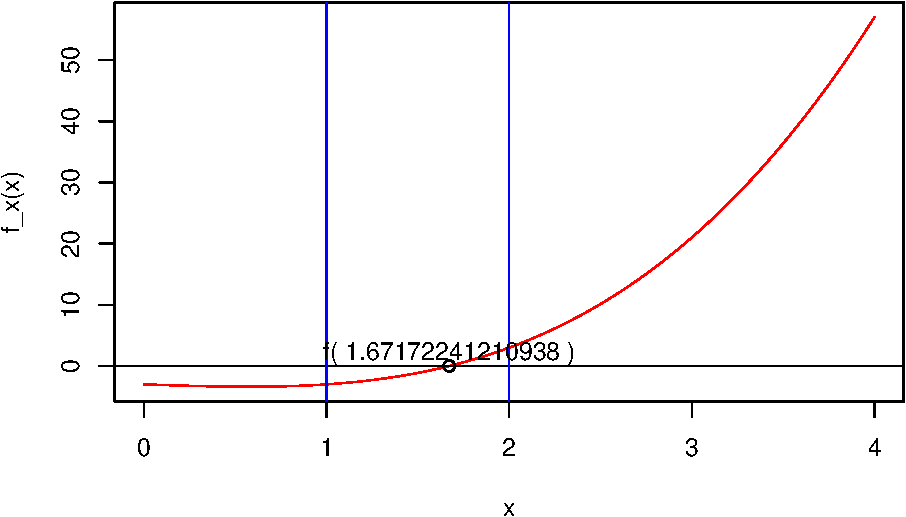
\includegraphics{Problem_Set_2_files/figure-latex/unnamed-chunk-2-1.pdf}

\paragraph{\texorpdfstring{2.) The function
\(f(x) = -3x^3 + 2e^{\frac{x^2}{2}} - 1\) has values of zero near
\(x=-0.5\) and
\(x=0.5\).}{2.) The function f(x) = -3x\^{}3 + 2e\^{}\{\textbackslash frac\{x\^{}2\}\{2\}\} - 1 has values of zero near x=-0.5 and x=0.5.}}\label{the-function-fx--3x3-2efracx22---1-has-values-of-zero-near-x-0.5-and-x0.5.}

\begin{enumerate}
\def\labelenumi{\alph{enumi}.}
\tightlist
\item
  What is the derivative of \(f\)? \textbf{Answer:}
\end{enumerate}

\[
\begin{aligned}
f(x) &= -3x^3 + 2e^{\frac{x^2}{2}} - 1 \\
f'(x) &= -9x^2 + 2xe^{\frac{x^2}{2}}
\end{aligned}
\]

\[
\boxed{
\text{Therefore, the derivative of } f \text{ is } -9x^2 + 2xe^{\frac{x^2}{2}}
}
\]

\begin{enumerate}
\def\labelenumi{\alph{enumi}.}
\setcounter{enumi}{1}
\tightlist
\item
  If you begin Newton's method at \(x = 1\), which root is reached? How
  many iterations to achieve an error less than \(10^{-5}\)?
  \textbf{Answer:}
\end{enumerate}

\begin{Shaded}
\begin{Highlighting}[]
\NormalTok{f\_x }\OtherTok{\textless{}{-}} \ControlFlowTok{function}\NormalTok{(x) \{ }\SpecialCharTok{{-}}\DecValTok{3}\SpecialCharTok{*}\NormalTok{x}\SpecialCharTok{\^{}}\DecValTok{3} \SpecialCharTok{+} \DecValTok{2} \SpecialCharTok{*} \FunctionTok{exp}\NormalTok{(x}\SpecialCharTok{\^{}}\DecValTok{2}\SpecialCharTok{/}\DecValTok{2}\NormalTok{) }\SpecialCharTok{{-}} \DecValTok{1}\NormalTok{ \}}
\NormalTok{f\_prime }\OtherTok{\textless{}{-}} \ControlFlowTok{function}\NormalTok{(x) \{ }\DecValTok{2} \SpecialCharTok{*}\NormalTok{ x }\SpecialCharTok{*} \FunctionTok{exp}\NormalTok{(x}\SpecialCharTok{\^{}}\DecValTok{2} \SpecialCharTok{/} \DecValTok{2}\NormalTok{) }\SpecialCharTok{{-}} \DecValTok{9} \SpecialCharTok{*}\NormalTok{ x}\SpecialCharTok{\^{}}\DecValTok{2}\NormalTok{ \}}
\NormalTok{tol }\OtherTok{\textless{}{-}} \FloatTok{0.00001}
\NormalTok{x\_curr }\OtherTok{\textless{}{-}} \DecValTok{1}

\NormalTok{newton\_table }\OtherTok{\textless{}{-}} \FunctionTok{list}\NormalTok{(}
  \StringTok{"Iteration"} \OtherTok{=} \FunctionTok{c}\NormalTok{(),}
  \StringTok{"x\_curr"} \OtherTok{=} \FunctionTok{c}\NormalTok{(),}
  \StringTok{"f\_x"} \OtherTok{=} \FunctionTok{c}\NormalTok{(),}
  \StringTok{"f\_prime"} \OtherTok{=} \FunctionTok{c}\NormalTok{(),}
  \StringTok{"x\_next"} \OtherTok{=} \FunctionTok{c}\NormalTok{(),}
  \StringTok{"Err."} \OtherTok{=} \FunctionTok{c}\NormalTok{()}
\NormalTok{)}

\CommentTok{\# Newton\textquotesingle{}s Method Algorithm}
\NormalTok{iters }\OtherTok{\textless{}{-}} \DecValTok{1}
\ControlFlowTok{repeat}\NormalTok{ \{}
\NormalTok{  f\_curr }\OtherTok{\textless{}{-}} \FunctionTok{f\_x}\NormalTok{(x\_curr)}
\NormalTok{  f\_prime\_curr }\OtherTok{\textless{}{-}} \FunctionTok{f\_prime}\NormalTok{(x\_curr)}
  
\NormalTok{  x\_next }\OtherTok{\textless{}{-}}\NormalTok{ x\_curr }\SpecialCharTok{{-}}\NormalTok{ f\_curr }\SpecialCharTok{/}\NormalTok{ f\_prime\_curr}
\NormalTok{  newton\_abs\_err }\OtherTok{\textless{}{-}} \FunctionTok{abs}\NormalTok{(x\_next }\SpecialCharTok{{-}}\NormalTok{ x\_curr)}
  
\NormalTok{  newton\_table}\SpecialCharTok{$}\NormalTok{Iteration }\OtherTok{\textless{}{-}} \FunctionTok{c}\NormalTok{(newton\_table}\SpecialCharTok{$}\NormalTok{Iteration, iters)}
\NormalTok{  newton\_table}\SpecialCharTok{$}\NormalTok{x\_curr }\OtherTok{\textless{}{-}} \FunctionTok{c}\NormalTok{(newton\_table}\SpecialCharTok{$}\NormalTok{x\_curr, x\_curr)}
\NormalTok{  newton\_table}\SpecialCharTok{$}\NormalTok{f\_x }\OtherTok{\textless{}{-}} \FunctionTok{c}\NormalTok{(newton\_table}\SpecialCharTok{$}\NormalTok{f\_x, f\_curr)}
\NormalTok{  newton\_table}\SpecialCharTok{$}\NormalTok{f\_prime }\OtherTok{\textless{}{-}} \FunctionTok{c}\NormalTok{(newton\_table}\SpecialCharTok{$}\NormalTok{f\_prime, f\_prime\_curr)}
\NormalTok{  newton\_table}\SpecialCharTok{$}\NormalTok{x\_next }\OtherTok{\textless{}{-}} \FunctionTok{c}\NormalTok{(newton\_table}\SpecialCharTok{$}\NormalTok{x\_next, x\_next)}
\NormalTok{  newton\_table}\SpecialCharTok{$}\NormalTok{Err. }\OtherTok{\textless{}{-}} \FunctionTok{c}\NormalTok{(newton\_table}\SpecialCharTok{$}\NormalTok{Err., newton\_abs\_err)}
  
  \ControlFlowTok{if}\NormalTok{ (newton\_abs\_err }\SpecialCharTok{\textless{}=}\NormalTok{ tol) \{}
    \ControlFlowTok{break}
\NormalTok{  \}}
  
\NormalTok{  x\_curr }\OtherTok{\textless{}{-}}\NormalTok{ x\_next}
\NormalTok{  iters }\OtherTok{\textless{}{-}}\NormalTok{ iters }\SpecialCharTok{+} \DecValTok{1}
\NormalTok{\}}

\NormalTok{newton\_table\_df }\OtherTok{\textless{}{-}} \FunctionTok{as.data.frame}\NormalTok{(newton\_table)}
\NormalTok{newton\_table\_df}
\end{Highlighting}
\end{Shaded}

\begin{verbatim}
##   Iteration    x_curr           f_x   f_prime    x_next         Err.
## 1         1 1.0000000 -7.025575e-01 -5.702557 0.8767996 1.232004e-01
## 2         2 0.8767996 -8.475879e-02 -4.343458 0.8572855 1.951413e-02
## 3         3 0.8572855 -2.005304e-03 -4.138476 0.8568009 4.845513e-04
## 4         4 0.8568009 -1.223134e-06 -4.133428 0.8568006 2.959127e-07
\end{verbatim}

\[
\boxed{\text{Therefore, the root is } 0.8568 \text{ when } x=1 {\text { and the number of iterations needed to achieve an error less than 10-5 is 4 iterations.}}}
\]

\begin{enumerate}
\def\labelenumi{\alph{enumi}.}
\setcounter{enumi}{2}
\tightlist
\item
  Begin Newton's method at another starting point to get the other zero.
  \textbf{Answer: Using the starting point} \(x=2\)
\end{enumerate}

\begin{Shaded}
\begin{Highlighting}[]
\NormalTok{x\_curr }\OtherTok{\textless{}{-}} \DecValTok{2}
\NormalTok{newton\_table\_2 }\OtherTok{\textless{}{-}} \FunctionTok{list}\NormalTok{(}
  \StringTok{"Iteration"} \OtherTok{=} \FunctionTok{c}\NormalTok{(),}
  \StringTok{"x\_curr"} \OtherTok{=} \FunctionTok{c}\NormalTok{(),}
  \StringTok{"f\_x"} \OtherTok{=} \FunctionTok{c}\NormalTok{(),}
  \StringTok{"f\_prime"} \OtherTok{=} \FunctionTok{c}\NormalTok{(),}
  \StringTok{"x\_next"} \OtherTok{=} \FunctionTok{c}\NormalTok{(),}
  \StringTok{"Err."} \OtherTok{=} \FunctionTok{c}\NormalTok{()}
\NormalTok{)}

\NormalTok{iters }\OtherTok{\textless{}{-}} \DecValTok{1}
\ControlFlowTok{repeat}\NormalTok{ \{}
\NormalTok{  f\_curr }\OtherTok{\textless{}{-}} \FunctionTok{f\_x}\NormalTok{(x\_curr)}
\NormalTok{  f\_prime\_curr }\OtherTok{\textless{}{-}} \FunctionTok{f\_prime}\NormalTok{(x\_curr)}
  
\NormalTok{  x\_next }\OtherTok{\textless{}{-}}\NormalTok{ x\_curr }\SpecialCharTok{{-}}\NormalTok{ f\_curr }\SpecialCharTok{/}\NormalTok{ f\_prime\_curr}
\NormalTok{  newton\_abs\_err }\OtherTok{\textless{}{-}} \FunctionTok{abs}\NormalTok{(x\_next }\SpecialCharTok{{-}}\NormalTok{ x\_curr)}
  
\NormalTok{  newton\_table\_2}\SpecialCharTok{$}\NormalTok{Iteration }\OtherTok{\textless{}{-}} \FunctionTok{c}\NormalTok{(newton\_table\_2}\SpecialCharTok{$}\NormalTok{Iteration, iters)}
\NormalTok{  newton\_table\_2}\SpecialCharTok{$}\NormalTok{x\_curr }\OtherTok{\textless{}{-}} \FunctionTok{c}\NormalTok{(newton\_table\_2}\SpecialCharTok{$}\NormalTok{x\_curr, x\_curr)}
\NormalTok{  newton\_table\_2}\SpecialCharTok{$}\NormalTok{f\_x }\OtherTok{\textless{}{-}} \FunctionTok{c}\NormalTok{(newton\_table\_2}\SpecialCharTok{$}\NormalTok{f\_x, f\_curr)}
\NormalTok{  newton\_table\_2}\SpecialCharTok{$}\NormalTok{f\_prime }\OtherTok{\textless{}{-}} \FunctionTok{c}\NormalTok{(newton\_table\_2}\SpecialCharTok{$}\NormalTok{f\_prime, f\_prime\_curr)}
\NormalTok{  newton\_table\_2}\SpecialCharTok{$}\NormalTok{x\_next }\OtherTok{\textless{}{-}} \FunctionTok{c}\NormalTok{(newton\_table\_2}\SpecialCharTok{$}\NormalTok{x\_next, x\_next)}
\NormalTok{  newton\_table\_2}\SpecialCharTok{$}\NormalTok{Err. }\OtherTok{\textless{}{-}} \FunctionTok{c}\NormalTok{(newton\_table\_2}\SpecialCharTok{$}\NormalTok{Err., newton\_abs\_err)}
  
  \ControlFlowTok{if}\NormalTok{ (newton\_abs\_err }\SpecialCharTok{\textless{}=}\NormalTok{ tol) \{}
    \ControlFlowTok{break}
\NormalTok{  \}}
  
\NormalTok{  x\_curr }\OtherTok{\textless{}{-}}\NormalTok{ x\_next}
\NormalTok{  iters }\OtherTok{\textless{}{-}}\NormalTok{ iters }\SpecialCharTok{+} \DecValTok{1}
\NormalTok{\}}

\NormalTok{newton\_table\_2\_df }\OtherTok{\textless{}{-}} \FunctionTok{as.data.frame}\NormalTok{(newton\_table\_2)}
\NormalTok{newton\_table\_2\_df}
\end{Highlighting}
\end{Shaded}

\begin{verbatim}
##   Iteration    x_curr           f_x    f_prime    x_next         Err.
## 1         1 2.0000000 -1.022189e+01 -6.4437756 0.4136804 1.586320e+00
## 2         2 0.4136804  9.662852e-01 -0.6389115 1.9260732 1.512393e+00
## 3         3 1.9260732 -9.653946e+00 -8.7690447 0.8251612 1.100912e+00
## 4         4 0.8251612  1.256128e-01 -3.8083693 0.8581445 3.298335e-02
## 5         5 0.8581445 -5.564475e-03 -4.1474310 0.8568029 1.341668e-03
## 6         6 0.8568029 -9.381960e-06 -4.1334481 0.8568006 2.269766e-06
\end{verbatim}

\[
\boxed{\text{Therefore, the root is } 0.8568 \text{ when } x=2}
\]

\paragraph{\texorpdfstring{3.) Use the function from no. 2 and find the
root using the secant method where \(x_0=0\) and \(x_1=1\). Use an error
tolerance of
\(\epsilon = 0.001\).}{3.) Use the function from no. 2 and find the root using the secant method where x\_0=0 and x\_1=1. Use an error tolerance of \textbackslash epsilon = 0.001.}}\label{use-the-function-from-no.-2-and-find-the-root-using-the-secant-method-where-x_00-and-x_11.-use-an-error-tolerance-of-epsilon-0.001.}

\begin{Shaded}
\begin{Highlighting}[]
\NormalTok{secant\_table }\OtherTok{\textless{}{-}} \FunctionTok{list}\NormalTok{(}
  \StringTok{"x\_prev"} \OtherTok{=} \FunctionTok{c}\NormalTok{(),}
  \StringTok{"x\_curr"} \OtherTok{=} \FunctionTok{c}\NormalTok{(),}
  \StringTok{"x\_next"} \OtherTok{=} \FunctionTok{c}\NormalTok{(),}
  \StringTok{"f\_x\_curr"} \OtherTok{=} \FunctionTok{c}\NormalTok{(),}
  \StringTok{"f\_x\_prev"} \OtherTok{=} \FunctionTok{c}\NormalTok{(),}
  \StringTok{"Error"} \OtherTok{=} \FunctionTok{c}\NormalTok{()}
\NormalTok{)}

\CommentTok{\# Secant Method Algorithm}
\NormalTok{MySecant }\OtherTok{\textless{}{-}} \ControlFlowTok{function}\NormalTok{(f, x\_prev, x, tol, table) \{}
\NormalTok{  f\_x\_prev }\OtherTok{\textless{}{-}} \FunctionTok{f}\NormalTok{(x\_prev)}
\NormalTok{  f\_x }\OtherTok{\textless{}{-}} \FunctionTok{f}\NormalTok{(x)}
  
\NormalTok{  num }\OtherTok{\textless{}{-}}\NormalTok{ x }\SpecialCharTok{{-}}\NormalTok{ x\_prev}
\NormalTok{  den }\OtherTok{\textless{}{-}}\NormalTok{ f\_x }\SpecialCharTok{{-}}\NormalTok{ f\_x\_prev}
  
\NormalTok{  next\_x }\OtherTok{\textless{}{-}}\NormalTok{ x }\SpecialCharTok{{-}}\NormalTok{ f\_x }\SpecialCharTok{*}\NormalTok{ (num }\SpecialCharTok{/}\NormalTok{ den)}
\NormalTok{  abs\_err }\OtherTok{\textless{}{-}} \FunctionTok{abs}\NormalTok{(next\_x }\SpecialCharTok{{-}}\NormalTok{ x)}
  
\NormalTok{  table}\SpecialCharTok{$}\NormalTok{x\_prev }\OtherTok{\textless{}{-}} \FunctionTok{c}\NormalTok{(table}\SpecialCharTok{$}\NormalTok{x\_prev, x\_prev)}
\NormalTok{  table}\SpecialCharTok{$}\NormalTok{x\_curr }\OtherTok{\textless{}{-}} \FunctionTok{c}\NormalTok{(table}\SpecialCharTok{$}\NormalTok{x\_curr, x)}
\NormalTok{  table}\SpecialCharTok{$}\NormalTok{x\_next }\OtherTok{\textless{}{-}} \FunctionTok{c}\NormalTok{(table}\SpecialCharTok{$}\NormalTok{x\_next, next\_x)}
\NormalTok{  table}\SpecialCharTok{$}\NormalTok{f\_x\_prev }\OtherTok{\textless{}{-}} \FunctionTok{c}\NormalTok{(table}\SpecialCharTok{$}\NormalTok{f\_x\_prev, f\_x\_prev)}
\NormalTok{  table}\SpecialCharTok{$}\NormalTok{f\_x\_curr }\OtherTok{\textless{}{-}} \FunctionTok{c}\NormalTok{(table}\SpecialCharTok{$}\NormalTok{f\_x\_curr, f\_x)}
\NormalTok{  table}\SpecialCharTok{$}\NormalTok{Error }\OtherTok{\textless{}{-}} \FunctionTok{c}\NormalTok{(table}\SpecialCharTok{$}\NormalTok{Error, abs\_err)}
  
  \ControlFlowTok{if}\NormalTok{ (abs\_err }\SpecialCharTok{\textless{}=}\NormalTok{ tol) \{}
    \FunctionTok{return}\NormalTok{(}\FunctionTok{list}\NormalTok{(}\AttributeTok{root =}\NormalTok{ next\_x, }\AttributeTok{table =}\NormalTok{ table))}
\NormalTok{  \} }\ControlFlowTok{else}\NormalTok{ \{}
    \FunctionTok{return}\NormalTok{(}\FunctionTok{MySecant}\NormalTok{(f, x, next\_x, tol, table))}
\NormalTok{  \}}
\NormalTok{\}}

\NormalTok{result }\OtherTok{\textless{}{-}} \FunctionTok{MySecant}\NormalTok{(f\_x, }\DecValTok{0}\NormalTok{, }\DecValTok{1}\NormalTok{, }\FloatTok{0.001}\NormalTok{, secant\_table)}

\NormalTok{secant\_table\_df }\OtherTok{\textless{}{-}} \FunctionTok{as.data.frame}\NormalTok{(result}\SpecialCharTok{$}\NormalTok{table)}
\NormalTok{secant\_table\_df}
\end{Highlighting}
\end{Shaded}

\begin{verbatim}
##      x_prev    x_curr    x_next      f_x_curr     f_x_prev        Error
## 1 0.0000000 1.0000000 0.5873517 -0.7025574586  1.000000000 4.126483e-01
## 2 1.0000000 0.5873517 0.8029441  0.7686449665 -0.702557459 2.155924e-01
## 3 0.5873517 0.8029441 0.8827930  0.2077417554  0.768644966 7.984897e-02
## 4 0.8029441 0.8827930 0.8549891 -0.1109815907  0.207741755 2.780394e-02
## 5 0.8827930 0.8549891 0.8567427  0.0074706294 -0.110981591 1.753559e-03
## 6 0.8549891 0.8567427 0.8568007  0.0002394906  0.007470629 5.807673e-05
\end{verbatim}

\[
\boxed{\text{Therefore, the root is } 0.857 \text{ when } x_0=0, x_1=1, \text{ and } \epsilon = 0.001 \text{ using the Secant Method}}
\]

\paragraph{4.) Consider the system of
equations:}\label{consider-the-system-of-equations}

\[
\begin{cases}
2x + 3y - z = 5 \\
4x - y + 2z = 6 \\
-3x + 2y + z = -4
\end{cases}
\]

\begin{enumerate}
\def\labelenumi{\alph{enumi}.}
\tightlist
\item
  Present the augmented matrix of the system. \textbf{Answer:}
\end{enumerate}

\[
\boxed{
\left(
\begin{array}{ccc|c}
2 & 3 & -1 & 5 \\
4 & -1 & 2 & 6 \\
-3 & 2 & 1 & -4
\end{array}
\right)
}
\]

\begin{enumerate}
\def\labelenumi{\alph{enumi}.}
\setcounter{enumi}{1}
\tightlist
\item
  Solve the system using \(Ax=LUx=Ly=b\) and round the final answer to 4
  decimal digits. \textbf{Answer:}
\end{enumerate}

\begin{Shaded}
\begin{Highlighting}[]
\NormalTok{LU }\OtherTok{\textless{}{-}} \ControlFlowTok{function}\NormalTok{(mat)\{}
\NormalTok{  upper }\OtherTok{\textless{}{-}}\NormalTok{ mat}
\NormalTok{  n }\OtherTok{\textless{}{-}} \FunctionTok{nrow}\NormalTok{(mat)}
\NormalTok{  lower }\OtherTok{\textless{}{-}} \FunctionTok{diag}\NormalTok{(n)}
  
  \ControlFlowTok{for}\NormalTok{(col }\ControlFlowTok{in} \DecValTok{1}\SpecialCharTok{:}\NormalTok{(n}\DecValTok{{-}1}\NormalTok{))\{}
    \ControlFlowTok{for}\NormalTok{(row }\ControlFlowTok{in}\NormalTok{ (col}\SpecialCharTok{+}\DecValTok{1}\NormalTok{)}\SpecialCharTok{:}\NormalTok{n)\{}
\NormalTok{      m }\OtherTok{\textless{}{-}}\NormalTok{ upper[row, col] }\SpecialCharTok{/}\NormalTok{ upper[col, col]}
\NormalTok{      lower[row, col] }\OtherTok{\textless{}{-}}\NormalTok{ m}
\NormalTok{      upper[row,] }\OtherTok{=}\NormalTok{ upper[row,] }\SpecialCharTok{{-}}\NormalTok{ m }\SpecialCharTok{*}\NormalTok{ upper[col,]}
      \FunctionTok{print}\NormalTok{(}\FunctionTok{sprintf}\NormalTok{(}\StringTok{"Row Operation: R\_\%d ← R\_\%d {-} (\%.2f)R\_\%d"}\NormalTok{, row, row, m, col))}
      \FunctionTok{print}\NormalTok{(}\StringTok{"Upper:"}\NormalTok{)}
      \FunctionTok{print}\NormalTok{(upper)}
      \FunctionTok{print}\NormalTok{(}\StringTok{"Lower:"}\NormalTok{)}
      \FunctionTok{print}\NormalTok{(lower)}
\NormalTok{    \}}
\NormalTok{  \}}
  
  \FunctionTok{return}\NormalTok{(}\FunctionTok{list}\NormalTok{(}\AttributeTok{L =}\NormalTok{ lower, }\AttributeTok{U =}\NormalTok{ upper))}
\NormalTok{\}}

\NormalTok{A }\OtherTok{=} \FunctionTok{matrix}\NormalTok{(}\FunctionTok{c}\NormalTok{(}\DecValTok{2}\NormalTok{, }\DecValTok{3}\NormalTok{, }\SpecialCharTok{{-}}\DecValTok{1}\NormalTok{, }\DecValTok{4}\NormalTok{, }\SpecialCharTok{{-}}\DecValTok{1}\NormalTok{, }\DecValTok{2}\NormalTok{, }\SpecialCharTok{{-}}\DecValTok{3}\NormalTok{, }\DecValTok{2}\NormalTok{, }\DecValTok{1}\NormalTok{), }\AttributeTok{nrow=}\DecValTok{3}\NormalTok{, }\AttributeTok{byrow=}\ConstantTok{TRUE}\NormalTok{)}
\NormalTok{b }\OtherTok{=} \FunctionTok{matrix}\NormalTok{(}\FunctionTok{c}\NormalTok{(}\DecValTok{5}\NormalTok{, }\DecValTok{6}\NormalTok{, }\SpecialCharTok{{-}}\DecValTok{4}\NormalTok{), }\AttributeTok{nrow=}\DecValTok{3}\NormalTok{, }\AttributeTok{byrow=}\ConstantTok{TRUE}\NormalTok{)}
\NormalTok{lu\_results }\OtherTok{=} \FunctionTok{LU}\NormalTok{(A)}
\end{Highlighting}
\end{Shaded}

\begin{verbatim}
## [1] "Row Operation: R_2 ← R_2 - (2.00)R_1"
## [1] "Upper:"
##      [,1] [,2] [,3]
## [1,]    2    3   -1
## [2,]    0   -7    4
## [3,]   -3    2    1
## [1] "Lower:"
##      [,1] [,2] [,3]
## [1,]    1    0    0
## [2,]    2    1    0
## [3,]    0    0    1
## [1] "Row Operation: R_3 ← R_3 - (-1.50)R_1"
## [1] "Upper:"
##      [,1] [,2] [,3]
## [1,]    2  3.0 -1.0
## [2,]    0 -7.0  4.0
## [3,]    0  6.5 -0.5
## [1] "Lower:"
##      [,1] [,2] [,3]
## [1,]  1.0    0    0
## [2,]  2.0    1    0
## [3,] -1.5    0    1
## [1] "Row Operation: R_3 ← R_3 - (-0.93)R_2"
## [1] "Upper:"
##      [,1] [,2]      [,3]
## [1,]    2    3 -1.000000
## [2,]    0   -7  4.000000
## [3,]    0    0  3.214286
## [1] "Lower:"
##      [,1]       [,2] [,3]
## [1,]  1.0  0.0000000    0
## [2,]  2.0  1.0000000    0
## [3,] -1.5 -0.9285714    1
\end{verbatim}

\begin{Shaded}
\begin{Highlighting}[]
\NormalTok{L }\OtherTok{=}\NormalTok{ lu\_results}\SpecialCharTok{$}\NormalTok{L}
\NormalTok{U }\OtherTok{=}\NormalTok{ lu\_results}\SpecialCharTok{$}\NormalTok{U}
\NormalTok{n }\OtherTok{\textless{}{-}} \FunctionTok{nrow}\NormalTok{(L)}

\CommentTok{\# Solving for y using Ly = b (Forward Substitution)}
\NormalTok{y }\OtherTok{\textless{}{-}} \FunctionTok{matrix}\NormalTok{(}\DecValTok{0}\NormalTok{, }\AttributeTok{nrow=}\DecValTok{3}\NormalTok{, }\AttributeTok{ncol=}\DecValTok{1}\NormalTok{)}

\ControlFlowTok{for}\NormalTok{(i }\ControlFlowTok{in} \DecValTok{1}\SpecialCharTok{:}\NormalTok{n)\{}
\NormalTok{  sum\_l }\OtherTok{\textless{}{-}} \DecValTok{0}
  \ControlFlowTok{if}\NormalTok{(i }\SpecialCharTok{\textgreater{}} \DecValTok{1}\NormalTok{)\{}
    \ControlFlowTok{for}\NormalTok{(j }\ControlFlowTok{in} \DecValTok{1}\SpecialCharTok{:}\NormalTok{(i}\DecValTok{{-}1}\NormalTok{))\{}
\NormalTok{      sum\_l }\OtherTok{\textless{}{-}}\NormalTok{ sum\_l }\SpecialCharTok{+}\NormalTok{ L[i,j] }\SpecialCharTok{*}\NormalTok{ y[j,}\DecValTok{1}\NormalTok{]}
\NormalTok{    \}}
\NormalTok{  \}}
\NormalTok{  y[i,}\DecValTok{1}\NormalTok{] }\OtherTok{\textless{}{-}}\NormalTok{ b[i,}\DecValTok{1}\NormalTok{] }\SpecialCharTok{{-}}\NormalTok{ sum\_l}
\NormalTok{\}}
\FunctionTok{print}\NormalTok{(}\FunctionTok{round}\NormalTok{(y, }\DecValTok{4}\NormalTok{))}
\end{Highlighting}
\end{Shaded}

\begin{verbatim}
##         [,1]
## [1,]  5.0000
## [2,] -4.0000
## [3,] -0.2143
\end{verbatim}

\begin{Shaded}
\begin{Highlighting}[]
\CommentTok{\# Solving for x using Ux = y (Backward Substitution)}
\NormalTok{x }\OtherTok{=} \FunctionTok{matrix}\NormalTok{(}\DecValTok{0}\NormalTok{, }\AttributeTok{nrow=}\DecValTok{3}\NormalTok{, }\AttributeTok{ncol=}\DecValTok{1}\NormalTok{)}

\ControlFlowTok{for}\NormalTok{(i }\ControlFlowTok{in} \DecValTok{3}\SpecialCharTok{:}\DecValTok{1}\NormalTok{)\{}
\NormalTok{  sum\_u }\OtherTok{\textless{}{-}} \DecValTok{0}
  \ControlFlowTok{if}\NormalTok{ (i }\SpecialCharTok{\textless{}}\NormalTok{ n) \{}
    \ControlFlowTok{for}\NormalTok{(j }\ControlFlowTok{in}\NormalTok{ (i}\SpecialCharTok{+}\DecValTok{1}\NormalTok{)}\SpecialCharTok{:}\NormalTok{n)\{}
\NormalTok{      sum\_u }\OtherTok{\textless{}{-}}\NormalTok{ sum\_u }\SpecialCharTok{+}\NormalTok{ U[i,j] }\SpecialCharTok{*}\NormalTok{ x[j,}\DecValTok{1}\NormalTok{]}
\NormalTok{    \}}
\NormalTok{  \}}
\NormalTok{  x[i,}\DecValTok{1}\NormalTok{] }\OtherTok{\textless{}{-}}\NormalTok{ (y[i,}\DecValTok{1}\NormalTok{] }\SpecialCharTok{{-}}\NormalTok{ sum\_u) }\SpecialCharTok{/}\NormalTok{ U[i,i]}
\NormalTok{\}}
\FunctionTok{print}\NormalTok{(}\FunctionTok{round}\NormalTok{(x, }\DecValTok{4}\NormalTok{))}
\end{Highlighting}
\end{Shaded}

\begin{verbatim}
##         [,1]
## [1,]  1.6667
## [2,]  0.5333
## [3,] -0.0667
\end{verbatim}

\[
\boxed{
\text{Therefore, the solution is } x = (1.6667, 0.5333, -0.0667)
}
\]

\begin{enumerate}
\def\labelenumi{\alph{enumi}.}
\setcounter{enumi}{2}
\tightlist
\item
  Find the residual vector if the correct solution is:
  \(x=1, y=2, z=-1\) \textbf{Answer:}
\end{enumerate}

\$\$

\begin{aligned}

r &= b - Ax \\
r &= 

\left(
\begin{array}{c}
5 \\ 6 \\ -4 
\end{array}
\right)

-

\left(
\begin{array}{ccc}
2 & 3 & -1 \\
4 & -1 & 2 \\
-3 & 2 & 1
\end{array}
\right)

\left(
\begin{array}{c}
1 \\ 2 \\ -1 
\end{array}
\right) \\

r &=

\left(
\begin{array}{c}
5 \\ 6 \\ -4 
\end{array}
\right)

-

\left(
\begin{array}{c}
9 \\ 0 \\ 0 
\end{array}
\right) \\

r &= 

\left(
\begin{array}{c}
-4 \\ 6 \\ -4 
\end{array}
\right)

\end{aligned}

\$\$

\[
\boxed{\text{Therefore, the residual vector is } (-4, 6, -4)}
\]

\paragraph{5.) Compute the Frobenius norm, maximum column sum, and
maximum row sum of the
matrix:}\label{compute-the-frobenius-norm-maximum-column-sum-and-maximum-row-sum-of-the-matrix}

\[
\left(
\begin{array}{ccc}
10.2 & 2.4 & 4.5 \\
-2.3 & 7.7 & 11.1 \\
-5.5 & -3.2 & 0.9
\end{array}
\right)
\]

\textbf{Answer:}

\[
\begin{aligned}
||A||_f &= \sqrt{(10.2)^2 + (-2.3)^2 + (-5.5)^2 + (2.4)^2 + (7.7)^2 + (-3.2)^2 + (4.5)^2 + (11.1)^2 + (0.9)^2} \\
||A||_f &= \sqrt{104.04 + 5.29 + 30.25 + 5.76 + 59.29 + 10.24 + 20.25 + 123.21 + 0.81} \\
||A||_f &= \sqrt{359.14} \\
||A||_f &= 18.95098942
\end{aligned}
\]

\[
\begin{aligned}
&\text{Maximum Column Sum} \\
\text{Col. 1} &= |10.2| + |-2.3| + |-5.5| = 18.0 \\
\text{Col. 2} &= |2.4| + |7.7| + |-3.2| = 13.3 \\
\text{Col. 3} &= |4.5| + |11.1| + |0.9| = 16.5 \\
\text{MaxColSum} &= max(18.0, 13.3, 16.5) \\
\text{MaxColSum} &= 18.0
\end{aligned}
\]

\[
\begin{aligned}
&\text{Maximum Row Sum} \\
\text{Row. 1} &= |10.2| + |2.4| + |4.5| = 17.1 \\
\text{Row. 2} &= |-2.3| + |7.7| + |11.1| = 21.1 \\
\text{Row. 3} &= |-5.5| + |-3.2| + |0.9| = 9.6 \\
\text{MaxRowSum} &= max(17.1, 21.1, 9.6) \\
\text{MaxRowSum} &= 21.1
\end{aligned}
\]

\[
\begin{aligned}
||A||_f &= 18.95098942 \text{, Frobenius Norm} \\
||A||_1 &= 18.0 \text{, Maximum column sum} \\
||A||_\infty &= 21.1 \text{, Maximum row sum}
\end{aligned}
\]

\paragraph{\texorpdfstring{6.) Solve the system of equations given in
no. 4, starting with the initial vector of
\([0,0,0]\):}{6.) Solve the system of equations given in no. 4, starting with the initial vector of {[}0,0,0{]}:}}\label{solve-the-system-of-equations-given-in-no.-4-starting-with-the-initial-vector-of-000}

\begin{Shaded}
\begin{Highlighting}[]
\CommentTok{\# Preprocessing the LUD matrices}
\NormalTok{A }\OtherTok{=} \FunctionTok{matrix}\NormalTok{(}\FunctionTok{c}\NormalTok{(}\DecValTok{2}\NormalTok{, }\DecValTok{3}\NormalTok{, }\SpecialCharTok{{-}}\DecValTok{1}\NormalTok{, }\DecValTok{4}\NormalTok{, }\SpecialCharTok{{-}}\DecValTok{1}\NormalTok{, }\DecValTok{2}\NormalTok{, }\SpecialCharTok{{-}}\DecValTok{3}\NormalTok{, }\DecValTok{2}\NormalTok{, }\DecValTok{1}\NormalTok{), }\AttributeTok{nrow=}\DecValTok{3}\NormalTok{, }\AttributeTok{byrow=}\ConstantTok{TRUE}\NormalTok{)}
\NormalTok{b }\OtherTok{=} \FunctionTok{matrix}\NormalTok{(}\FunctionTok{c}\NormalTok{(}\DecValTok{5}\NormalTok{, }\DecValTok{6}\NormalTok{, }\SpecialCharTok{{-}}\DecValTok{4}\NormalTok{), }\AttributeTok{nrow=}\DecValTok{3}\NormalTok{, }\AttributeTok{byrow=}\ConstantTok{TRUE}\NormalTok{)}

\CommentTok{\# This function returns the Lower Triangle, Upper Triangle, and Diagonal Matrices}
\NormalTok{LUD\_jacobi }\OtherTok{\textless{}{-}} \ControlFlowTok{function}\NormalTok{(mat)\{}
\NormalTok{  n }\OtherTok{\textless{}{-}} \FunctionTok{nrow}\NormalTok{(mat)}
\NormalTok{  lower }\OtherTok{\textless{}{-}} \FunctionTok{matrix}\NormalTok{(}\DecValTok{0}\NormalTok{, }\AttributeTok{nrow=}\NormalTok{n, }\AttributeTok{ncol=}\NormalTok{n)}
\NormalTok{  upper }\OtherTok{\textless{}{-}} \FunctionTok{matrix}\NormalTok{(}\DecValTok{0}\NormalTok{, }\AttributeTok{nrow=}\NormalTok{n, }\AttributeTok{ncol=}\NormalTok{n)}
\NormalTok{  diag  }\OtherTok{\textless{}{-}} \FunctionTok{matrix}\NormalTok{(}\DecValTok{0}\NormalTok{, }\AttributeTok{nrow=}\NormalTok{n, }\AttributeTok{ncol=}\NormalTok{n)}
  
  \ControlFlowTok{for}\NormalTok{(i }\ControlFlowTok{in} \DecValTok{1}\SpecialCharTok{:}\NormalTok{n)\{}
\NormalTok{    diag[i,i] }\OtherTok{\textless{}{-}}\NormalTok{ mat[i,i]}
\NormalTok{    j }\OtherTok{\textless{}{-}} \DecValTok{1}
    \ControlFlowTok{while}\NormalTok{(j }\SpecialCharTok{\textless{}=}\NormalTok{ (i}\DecValTok{{-}1}\NormalTok{))\{}
\NormalTok{      lower[i,j] }\OtherTok{\textless{}{-}}\NormalTok{ mat[i,j]}
\NormalTok{      upper[j,i] }\OtherTok{\textless{}{-}}\NormalTok{ mat[j,i]}
\NormalTok{      j }\OtherTok{\textless{}{-}}\NormalTok{ j }\SpecialCharTok{+} \DecValTok{1} 
\NormalTok{    \}}
\NormalTok{  \}}
  
  \FunctionTok{return}\NormalTok{(}\FunctionTok{list}\NormalTok{(}\AttributeTok{L =}\NormalTok{ lower, }\AttributeTok{U =}\NormalTok{ upper, }\AttributeTok{D =}\NormalTok{ diag))}
\NormalTok{\}}

\NormalTok{LUD\_results }\OtherTok{\textless{}{-}} \FunctionTok{LUD\_jacobi}\NormalTok{(A)}

\CommentTok{\# Lower Triangle}
\NormalTok{L }\OtherTok{\textless{}{-}}\NormalTok{ LUD\_results}\SpecialCharTok{$}\NormalTok{L}
\NormalTok{L}
\end{Highlighting}
\end{Shaded}

\begin{verbatim}
##      [,1] [,2] [,3]
## [1,]    0    0    0
## [2,]    4    0    0
## [3,]   -3    2    0
\end{verbatim}

\begin{Shaded}
\begin{Highlighting}[]
\CommentTok{\# Upper Triangle}
\NormalTok{U }\OtherTok{\textless{}{-}}\NormalTok{ LUD\_results}\SpecialCharTok{$}\NormalTok{U}
\NormalTok{U}
\end{Highlighting}
\end{Shaded}

\begin{verbatim}
##      [,1] [,2] [,3]
## [1,]    0    3   -1
## [2,]    0    0    2
## [3,]    0    0    0
\end{verbatim}

\begin{Shaded}
\begin{Highlighting}[]
\CommentTok{\# Diagonal}
\NormalTok{D }\OtherTok{\textless{}{-}}\NormalTok{ LUD\_results}\SpecialCharTok{$}\NormalTok{D}
\NormalTok{D}
\end{Highlighting}
\end{Shaded}

\begin{verbatim}
##      [,1] [,2] [,3]
## [1,]    2    0    0
## [2,]    0   -1    0
## [3,]    0    0    1
\end{verbatim}

\begin{enumerate}
\def\labelenumi{\alph{enumi}.}
\tightlist
\item
  Solve using the Jacobi method with 2-digit precision. \textbf{Answer:
  The system of equations cannot guarantee convergence using the Jacobi
  Method since it violates the condition wherein the diagonal values
  must be greater than or equal to the sum of its non-diagonal entries
  in the same row. Even, rearranging the rows to satisfy the diagonally
  dominant condition is futile.} \[
  \boxed{
  \text{Therefore, it cannot be solved using the Jacobi Method}
  }
  \]
\end{enumerate}

\begin{Shaded}
\begin{Highlighting}[]
\CommentTok{\# Example Divergence with 5 iterations (Jacobi Method)}
\NormalTok{x }\OtherTok{\textless{}{-}} \FunctionTok{matrix}\NormalTok{(}\DecValTok{0}\NormalTok{, }\AttributeTok{nrow=}\DecValTok{3}\NormalTok{, }\AttributeTok{ncol=}\DecValTok{1}\NormalTok{)}
\ControlFlowTok{for}\NormalTok{(i }\ControlFlowTok{in} \DecValTok{1}\SpecialCharTok{:}\DecValTok{5}\NormalTok{)\{}
\NormalTok{  x }\OtherTok{\textless{}{-}}\NormalTok{ (}\SpecialCharTok{{-}}\DecValTok{1}\SpecialCharTok{*}\FunctionTok{solve}\NormalTok{(D)) }\SpecialCharTok{\%*\%}\NormalTok{ (L }\SpecialCharTok{+}\NormalTok{ U) }\SpecialCharTok{\%*\%}\NormalTok{ x }\SpecialCharTok{+} \FunctionTok{solve}\NormalTok{(D) }\SpecialCharTok{\%*\%}\NormalTok{ b}
  \FunctionTok{print}\NormalTok{(}\FunctionTok{round}\NormalTok{(x, }\AttributeTok{digits =} \DecValTok{2}\NormalTok{))}
\NormalTok{\}}
\end{Highlighting}
\end{Shaded}

\begin{verbatim}
##      [,1]
## [1,]  2.5
## [2,] -6.0
## [3,] -4.0
##      [,1]
## [1,]  9.5
## [2,] -4.0
## [3,] 15.5
##       [,1]
## [1,] 16.25
## [2,] 63.00
## [3,] 32.50
##        [,1]
## [1,] -75.75
## [2,] 124.00
## [3,] -81.25
##         [,1]
## [1,] -224.12
## [2,] -471.50
## [3,] -479.25
\end{verbatim}

\begin{enumerate}
\def\labelenumi{\alph{enumi}.}
\setcounter{enumi}{1}
\tightlist
\item
  Solve using Gauss-Seidel method with 2-digit precision.
  \textbf{Answer: Similar with the Jacobi Method, The system of
  equations cannot guarantee convergence using the Gauss-Seidel Method
  since it violates the condition wherein the diagonal values must be
  greater than or equal to the sum of its non-diagonal entries in the
  same row. Even, rearranging the rows to satisfy the diagonally
  dominant condition is futile.}
\end{enumerate}

\[
\boxed{
\text{Therefore, it cannot be solved using the Gauss-Seidel Method}
}
\]

\begin{Shaded}
\begin{Highlighting}[]
\CommentTok{\# Example Divergence with 5 iterations (Gauss{-}Seidel Method)}
\NormalTok{x }\OtherTok{\textless{}{-}} \FunctionTok{matrix}\NormalTok{(}\DecValTok{0}\NormalTok{, }\AttributeTok{nrow=}\DecValTok{3}\NormalTok{, }\AttributeTok{ncol=}\DecValTok{1}\NormalTok{)}
\ControlFlowTok{for}\NormalTok{(i }\ControlFlowTok{in} \DecValTok{1}\SpecialCharTok{:}\DecValTok{5}\NormalTok{)\{}
\NormalTok{  x }\OtherTok{\textless{}{-}} \SpecialCharTok{{-}}\DecValTok{1} \SpecialCharTok{*} \FunctionTok{solve}\NormalTok{(L }\SpecialCharTok{+}\NormalTok{ D) }\SpecialCharTok{\%*\%}\NormalTok{ U }\SpecialCharTok{\%*\%}\NormalTok{ x }\SpecialCharTok{+} \FunctionTok{solve}\NormalTok{(L }\SpecialCharTok{+}\NormalTok{ D) }\SpecialCharTok{\%*\%}\NormalTok{ b}
  \FunctionTok{print}\NormalTok{(}\FunctionTok{round}\NormalTok{(x, }\AttributeTok{digits =} \DecValTok{2}\NormalTok{))}
\NormalTok{\}}
\end{Highlighting}
\end{Shaded}

\begin{verbatim}
##      [,1]
## [1,]  2.5
## [2,]  4.0
## [3,] -4.5
##        [,1]
## [1,]  -5.75
## [2,] -38.00
## [3,]  54.75
##         [,1]
## [1,]   86.88
## [2,]  451.00
## [3,] -645.38
##          [,1]
## [1,]  -996.69
## [2,] -5283.50
## [3,]  7572.94
##           [,1]
## [1,]  11714.22
## [2,]  61996.75
## [3,] -88854.84
\end{verbatim}

\begin{enumerate}
\def\labelenumi{\alph{enumi}.}
\setcounter{enumi}{2}
\tightlist
\item
  Solve for \(\overline{e}\) if the true solution is: \(x=1, y=2, z=-1\)
  \textbf{Answer: Using the residual from no. 4,}
\end{enumerate}

\begin{Shaded}
\begin{Highlighting}[]
\NormalTok{A }\OtherTok{\textless{}{-}} \FunctionTok{matrix}\NormalTok{(}\FunctionTok{c}\NormalTok{(}\DecValTok{2}\NormalTok{, }\DecValTok{3}\NormalTok{, }\SpecialCharTok{{-}}\DecValTok{1}\NormalTok{, }\DecValTok{4}\NormalTok{, }\SpecialCharTok{{-}}\DecValTok{1}\NormalTok{, }\DecValTok{2}\NormalTok{, }\SpecialCharTok{{-}}\DecValTok{3}\NormalTok{, }\DecValTok{2}\NormalTok{, }\DecValTok{1}\NormalTok{), }\AttributeTok{nrow=}\DecValTok{3}\NormalTok{, }\AttributeTok{byrow=}\ConstantTok{TRUE}\NormalTok{)}
\NormalTok{r }\OtherTok{\textless{}{-}} \FunctionTok{matrix}\NormalTok{(}\FunctionTok{c}\NormalTok{(}\SpecialCharTok{{-}}\DecValTok{4}\NormalTok{, }\DecValTok{6}\NormalTok{, }\SpecialCharTok{{-}}\DecValTok{4}\NormalTok{), }\AttributeTok{nrow=}\DecValTok{3}\NormalTok{, }\AttributeTok{byrow=}\ConstantTok{TRUE}\NormalTok{)}
\NormalTok{e }\OtherTok{\textless{}{-}} \FunctionTok{solve}\NormalTok{(A) }\SpecialCharTok{\%*\%}\NormalTok{ r}
\FunctionTok{round}\NormalTok{(}\FunctionTok{abs}\NormalTok{(e), }\DecValTok{4}\NormalTok{)}
\end{Highlighting}
\end{Shaded}

\begin{verbatim}
##        [,1]
## [1,] 0.6667
## [2,] 1.4667
## [3,] 0.9333
\end{verbatim}

\[
\boxed{
\text{Therefore, } \overline{e} = (0.6667, 1.4667, 0.9333)
}
\]

\end{document}
